{
  \newmdenv[tikzsetting={draw=black,fill=white,fill opacity=0.7, line width=4pt},backgroundcolor=none,leftmargin=0,rightmargin=0,innertopmargin=4pt,skipbelow=\baselineskip,%
  skipabove=\baselineskip]{TitleBoxParametricity}

  \usebackgroundtemplate{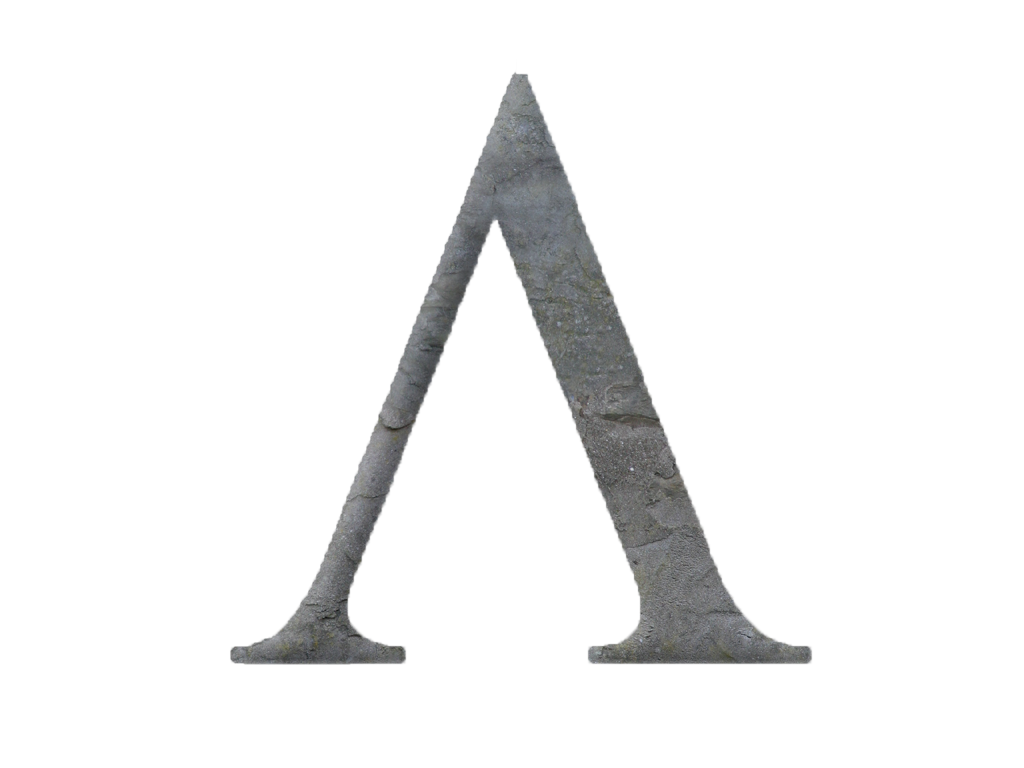
\includegraphics[width=1.0\paperwidth]{image/title-background.png}}

  \begin{frame}[plain] 
  \title{Parametricity}
  \subtitle{types are documentation}
  
  \vspace{3em}

  \begin{TitleBoxParametricity}
    \begin{center}
    {\Large \inserttitle}
    \end{center}
  \end{TitleBoxParametricity}

  \end{frame}
}


\begin{frame}
\frametitle{Parametricity}
\begin{block}{Parametricity, or Theorems for Free, is}
a technique described by Wadler\cite{wadler1989theorems} that gives rise to many practical consequences.
\end{block}
\end{frame}


\begin{frame}
\frametitle{Parametricity}
\begin{block}{One practical consequence of parametricity is that}
Types, by exploiting generalisation, may be utilised to document code and that documentation never goes out of date.
\end{block}
\end{frame}


\begin{frame}
\frametitle{Parametricity}
\begin{center}
Many nutty things have been said about static typing \ldots
\end{center}
\begin{center}
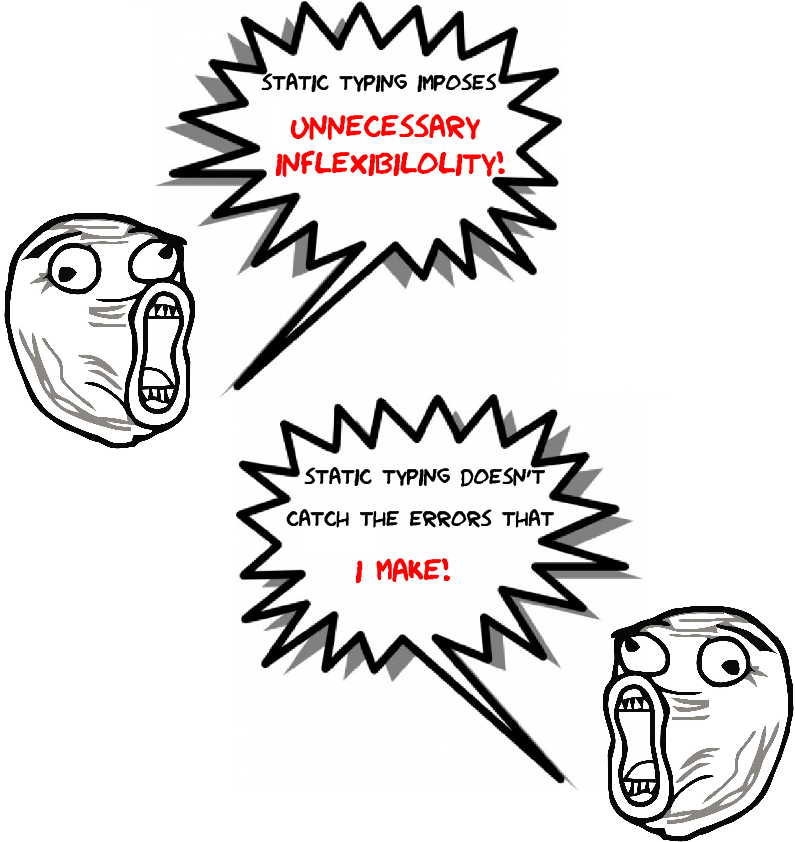
\includegraphics[width=0.5\paperwidth]{image/static-typing-nutty.png}
\end{center}
\end{frame}

{
\usebackgroundtemplate{
\begin{tikzpicture}[remember picture,overlay]
  \coordinate (aa) at ($(a1)+(-1,7.5)$);
  \node[right] at (aa) {
\includegraphics[height=1cm]{image/book-small.png}};
\end{tikzpicture}
}

\begin{frame}
\frametitle{Parametricity}
\begin{block}{\ldots including this one time}
a neurotic colleague insisted that static typing is terrible \ldots
\end{block}
\end{frame}


\begin{frame}[fragile]
\frametitle{Parametricity}
\ldots because you have to write messy types all the time!
\begin{lstlisting}[style=python,mathescape]
`int x`
x = 3
`String y`
y = "abc"
`(String, Int) a`
a = ("xyz", 9)
`[Int] b`
b = [1,4,9,16,x]
\end{lstlisting}
\end{frame}


\begin{frame}[fragile]
\frametitle{Parametricity}
So I took the Python source file
\begin{lstlisting}[style=python,mathescape]
x = 3
y = "abc"
a = ("xyz", 9)
b = [1,4,9,16,x]
\end{lstlisting}
\end{frame}


\begin{frame}[fragile]
\frametitle{Parametricity}
\ldots and loaded it into the Glasgow Haskell Compiler repl
\begin{lstlisting}
> ln -s soneat.py notypes.hs
> ghci notypes.hs
\end{lstlisting}
\end{frame}

}


\begin{frame}
\frametitle{Parametricity}
\begin{block}{The goal is to tell you about}
a more subtle, and rarely discussed, advantage that is available by appropriately exploiting types
\end{block}
\tiny{not so much to engage the static typing debate itself}
\end{frame}


\begin{frame}
\frametitle{Parametricity}
\framesubtitle{Theorems for Free!}
\begin{block}{Philip Wadler \cite{wadler1989theorems} tells us:}
\begin{quotation}
Write down the definition of a polymorphic function on a piece of paper. Tell me its type, but be careful not to let me see the function's definition. I will tell you a theorem that the function satisfies.

The purpose of this paper is to explain the trick.
\end{quotation}
\end{block}
\end{frame}


\begin{frame}
\frametitle{Totality}
\framesubtitle{Fast and loose reasoning is morally correct}
\begin{block}{Danielsson, Hughes, Jansson \& Gibbons \cite{danielsson2006fast} tell us:}
\begin{quotation}
Functional programmers often reason about programs as if
they were written in a total language, expecting the results
to carry over to non-total (partial) languages. We justify
such reasoning.
\end{quotation}
\end{block}
\end{frame}


\begin{frame}[fragile]
\frametitle{Parametricity}
\begin{block}{What if I told you}
\begin{quotation}
There exists a function that takes a list of some element type and returns a list of elements of that same type? 
\end{quotation}
\begin{lstlisting}[style=haskell]
function :: [a] -> [a]
\end{lstlisting}
\end{block}
\end{frame}


\begin{frame}[fragile]
\frametitle{Parametricity}
\begin{block}{I observe that}
there is nothing else to know about this element type
\end{block}
Its declared structure is \emph{universally quantified}
\end{frame}


\begin{frame}
\frametitle{Parametricity}
\begin{block}{On this information alone, I can $\therefore$ conclude that}
\textbf{Theorem} every element in the result appears in the input
\end{block}
\end{frame}


\begin{frame}
\frametitle{Parametricity}
\framesubtitle{Fast and Loose Reasoning}
\begin{block}{Morally Correct?}
What does it mean to ``reason as if we were in a total language, expecting the results to carry over to non-total languages''?
\end{block}
\end{frame}


\begin{frame}
\frametitle{Parametricity}
\framesubtitle{Fast and Loose Reasoning}
\begin{block}{It means we can ``morally'' exclude logical-inconsistencies $\bot$}
\begin{itemize}
  \item Type-case (e.g. \lstinline{is})
  \item Type-cast
  \item Type-value (e.g. \lstinline{type})
  \item unsafe universal functions e.g. \lstinline{str}, \lstinline{int}
  \item side-effects
  \item \lstinline{None} or \lstinline{null}
  \item exceptions
  \item Infinite recursion
\end{itemize}
\end{block}
\end{frame}


\begin{frame}
\frametitle{Parametricity}
\framesubtitle{Fast and Loose Reasoning}
\begin{block}{Some non-total systems do not have these $\bot$ values anyway}
\begin{itemize}
  \item \sout{Type-case e.g. (\lstinline{is})}
  \item \sout{Type-cast}
  \item \sout{Type-value e.g. (\lstinline{type})}
  \item \sout{unsafe universal functions e.g. \lstinline{str}, \lstinline{int}}
  \item \sout{side-effects}
  \item \sout{\lstinline{None} or \lstinline{null}}
  \item exceptions
  \item Infinite recursion
\end{itemize}
\end{block}
\end{frame}


\begin{frame}[fragile]
\frametitle{Parametricity}
\framesubtitle{Fast and Loose Reasoning}
\begin{block}{On the basis of fast and loose reasoning}
Can we invalidate the theorem, \textbf{every element in the result appears in the input}?
\end{block}
\begin{lstlisting}[style=haskell]
function :: [a] -> [a]
\end{lstlisting}
\end{frame}


\begin{frame}
\frametitle{Parametricity}
\begin{block}{OK, so we have machine-checked documentation, but}
How do we know what this function does exactly?
\end{block}
\end{frame}


\begin{frame}
\frametitle{Parametricity}
\begin{block}{We can write unit tests}
but not your laborious and clumsy kind
\end{block}
\end{frame}


\begin{frame}[fragile]
\frametitle{Parametricity}
\begin{block}{Specification-based tests or universally quantified properties\cite{claessen2011quickcheck}}
\begin{itemize}
  \item<1-> \lstinline[style=haskell,mathescape]{$\forall$ x. function [x] == [x]}
  \item<1-> \lstinline[style=haskell,mathescape]{$\forall$ x y. function (x ++ y) == function y ++ function x}
  \item<2-> Reminder: \lstinline{function :: [a] -> [a]}
  \item<2-> Now what does our \lstinline{function} do?
\end{itemize}
\end{block}
\end{frame}


\begin{frame}[fragile]
\frametitle{Parametricity}
\begin{block}{More theorems for free}
\begin{itemize}
  \item<1-> comp :: (a -> b) -> (b -> c) -> (a -> c)
  \item<2-> choose :: (a, a) -> a
\end{itemize}
\begin{lstlisting}
\end{lstlisting}
\end{block}
\end{frame}
